\documentclass[]{article}
\usepackage{amsmath} 
\usepackage{natbib}
\usepackage{graphicx}
\usepackage{caption}
\begin{document}

\title{Site-Heterogeneous Character Change Models for Morphology}
\author{Wright, Pett, Students, Heath}
\date{Today}
\maketitle

\section{Abstract}

Morphological data is challenging to model due to the complexity of morphological characters relative to nucleotide sequence or amino acid characters. 
The Mk model is the most commonly-used model for incorporating morphology in maximum likelihood and Bayesian work.
This model is a generalization of the Jukes-Cantor model, assumes that there is an equal rate of forward and backwards transitions in morphological traits.
In this study, we explore the use of models that allow asymmetrical transition rates.
We use an expanded combined set of two ant (Formicidae) data matrices, composed of one matrix of extinct and extant ants and one matrix of extant ants to estimate a phylogeny for the group.
In particular, we examine the use of two models to allow the equilibrium character frequency to vary. 
One model, a Beta prior on state frequencies is similar to a model implemented in MrBayes and can be used to allow asymmetrical transition rates in binary characters.
We also describe a Dirichlet model to allow asymmetrical transitions in multistate characters.
These two models can be used to explicitly model different character frequencies within one dataset, as opposed to assuming a single common mechanism with respect to among character frequency variation.

\section{Introduction}
\subsection{Bayesian Modeling of Morphology}
	Recent interest in using Bayesian methods to model morphological evolution to estimate phylogenetic trees has spurred many studies into how well the existing phylogenetic models perform, particularly in relation to parsimony methods.
	However, there has been little work expanding the toolkit of methods available to researchers estimating trees from morphological data. 
	The most common way to perform likelihood or Bayesian phylogenetic analysis using discrete morphological data is by applying a model of morphological evolution called the Mk model.
	Many workers using morphological data have raised questions about the realism of this model.
	In this paper, we will discuss methodological advancements aimed at improving the realism of the model. \par
	The Mk model was introduced by Lewis in 2001.
	As a generalization of the Jukes-Cantor model, it makes the same set of assumptions: that change between any two or more states  is equally likely, that the stationary character frequencies of every character are the same, and that each character is always in one of \textit{k} known states.
	The model also makes the Markovian assumption that a character can change instantaneously, regardless of previous states, and can change multiply along a branch. 
	Any one of these assumptions may strike a reader as problematic for their particular dataset. \par
	Heterogeneity in the evolutionary process is difficult to accommodate in morphological data. 
	Making concrete \textit{a priori} statements about the relative probabilities of transitions between character states in a morphological character matrix is challenging. 
	Unlike a matrix of nucleotide characters, in which a state carries common meaning across sites, a `1' state at one character may represent a derived state requiring many underlying genetic changes.
	At another character, it could represent a state requiring only one underlying genetic change.
	Characters can also differ in meanings with respect to whether they are coded as ancestral or derived.
	If a matrix was coded with respect to specific outgroups, often the outgroup will mostly have a `0' state, with ingroup taxa having typically having state `1' or higher, implying a highly one-directional transition matrix.
	This may not be the case for composite matrices or matrices coded without specific reference to an outgroup or character polarities.
	This lack of common meaning limits a researcher's ability to specify a model to apply to the whole matrix.
	This complicates researchers' ability to specify unique $\alpha$ parameters to the Q-matrix, or to apply multiple Q-matrices across the dataset.
	While the basic model is very simple, some elaborations of the model are common.
	Assumptions about character evolution, such as ordering, have been common in parsimony analysis, and can be accommodated under the Mk model. 
	This is a stark contrast to molecular data, in which base pairs or amino acid residues are generally assumed to have similar properties across an alignment, and exceptions are often defined with respect to known features, such as stem and loop domains. 
\par
Prior work extending the Mk model has focused on relaxing the assumption of equal character frequencies at stationarity.
MrBayes implemented a parameter called the Symmetric Dirichlet Hyperprior, which allowed users to place a prior or hyperprior on state frequencies. 
In most likelihood models of character or sequence evolution, the probability of observing a change in a character is dependent not only on the probability of change from this character to another, but on the frequency of the starting character.
Even if a character has a low probability of changing, change in that character may still be observed many times if the stationary frequency of that character is high (i.e., the character state is observed many times). 
Likewise, a highly probable changes may be seen relatively rarely if the starting character is observed rarely. 
Therefore, relaxing the assumption of equal stationary frequencies has been a way of changing the probabilities of observing different changes without making explicit \textit{a priori} statements about transition probabilities. \par
In the case of binary data, MrBayes implemented a Beta prior (the Dirichlet is a generalization of the Beta distribution for non-binary data), which operated in a fashion similar to gamma-distributed rate variation: the Beta distribution is discretized into a user-specified number of categories, the median forward and backward transition rate are calculated for each category by multiplying together the exchangeability and the character state frequency, and the likelihood of the character is calculated over each category and summed to form the total likelihood. 
For binary data, the state frequencies are integrated out of the likelihood, making the symmetric Dirichlet hyperprior actually a prior.
For multistate data, the state frequencies are fit via MCMC.
The parameter was referred to as a hyperprior because users can place a distribution on the parameter to the Beta distribution, and because the state frequencies are not integrated out of the likelihood function for multistate data. 
As implemented in MrBayes, the Beta distribution was assumed to be symmetric, meaning that if there was a class of characters for which the stationary frequency of 0 is high, there would also be corresponding class of characters for which the stationary frequency of 1 is high.
A formal description for the mathematics of the model was never published, and some of the mechanisms of operation remain unclear. 
\par
This is a very useful model extension for morphological evolution.
There are clear contexts to improve this concept by borrowing from the molecular literature.
The CAT model of Lartillot represents one way forward. 
This model, implemented in PhyloBayes, uses a Dirichlet process prior to assign individual sites to categories, which differ in their stationary frequencies. 
In this model, the number of such categories that describe the data is a free parameter. 
The use of a Dirichlet prior allows for flexibility in the number of states, as opposed to a Beta prior which is limited to binary data.
However, many datasets that have been analyzed under the CAT model are phylogenomic datasets of thousands of loci, as compared to data-limited morphology datasets.\par
In RevBayes, we have implemented a number of useful extensions to the Dirichlet prior of MrBayes, and a constrained version of the CAT model. 
Our extension to the symmetric Beta prior allows for the Beta distribution to be asymmetrical.
This removes the need for there to be equal numbers of characters with high stationary frequencies for a character state as there are characters with low stationary frequencies for that same character state.
Our CAT-like model (hereafter Site-Heterogeneous Discrete Morphology (SDHM) model) is a finite mixture model that allows characters to fit into a user-defined number of character categories that differ in their stationary frequencies. 
The bins draw their stationary frequencies from a Dirichlet to accommodate multistate data. 
A mathematical descriptionf of this model can be found in the methods section. \par

\subsection{Morphological Phylogeny of the Formicidae}

To test the efficacy of our analytical techniques, we use an ant dataset created from datasets from Barden and Grimaldi and one from Keller.
Ants are ecologically crucial organisms as both interacting partners for a variety of plants and animals, and as shapers of the ecosystem via soil cycling and nest building.
As such, they have attracted much work in the world of molecular systematics.
Ants have also have a rich fossil record, with most subfamilies being represented. 
This fossil record has been used for systematic work, as well as a variety of other ecological and evolutionary questions.\par
The monophyly of major subfamilies has been consistently supported by most molecular studies, with the exception of the Cerapachyinae. 
Molecular systematics had originally shaken up the ant tree of life considerably, breaking up clades considered to be monophyletic based on morphological work.
For example, based on morphological work, six current subfamilies had been previously considered to be a single subfamily, the Ponerinae, until molecular evidence indicated that two of the clades (Ectatomminae and Heteroponerinae) within that subfamily were demonstrated to be more closely related to other ants on the tree.
The Ponerinae was then broken into six distinct subfamilies, one of which is also called Ponerinae. 
Recent molecular work has continued to support these six subfamilies as monophyletic, though their relationships to one another remain poorly supported. \par
Excellent morphological matrices on the ingroup of the Formicidae have been available since the early '70s. 
Recent morphological matrices have expanded the sampling of ants from in the large Ponerine family, which was previously undersampled.
Sampling of fossil ants was also expanded to include specimens from the Cretaceous.
These ants were concluded to be stem lineages, and some did not demonstrate any particular taxonomic affinity based on character data and phylogenetic placement. 
Even with expanded taxon sampling in the Ponerinae, there is still conflict between the molecular and morphological estimates of phylogenetic relationships. 
Absent inputs of additional information, such as clade constraints, the trees are also substantially unresolved. \par
In this study, we combine the extant matrices of Keller, and the extinct-extant matrix of Barden and Grimaldi to expand the taxon and character sampling.  
This dataset has interesting properties.
Because there are stem ant lineages represented, there are taxa that have characteristics that are lost after the divergence of the stem lineages.
This extremely one-sided loss structure violates the Mk model assumption of equal transition rates. 
We would expect for these characters to be better modeled by a model that can accommodate asymmetrical transition rates.
Some apomorphies of the ant group are also gained after the divergence of the stem lineages, which also violates the assumption of equal change probabilities.
Because of these model violations, this dataset is an excellent test case for models that relax assumptions of the Mk model. \par
We use Bayes Factor model selection to assess the fit of these relaxed models to the data.
Using this dataset, we strongly support that the use of models that relax key assumptions of the Mk model can greatly improve the fit of the model to the data.
We also perform simulations to demonstrate that the true number of transition rate asymmetry categories is detectable from the data, and that using an appropriately-specified model of morphological evolution is less likely to lead to incorrect phylogenetic inference than a correctly specified model.\par
However, the morphological tree of ants remains poorly-resolved, consistent with prior morphological work in the group.
We do, however, support the monophyly of what  has been considered the crown group of ants, and support a monophyletic Haidomyrmicine ants, as in Barden and Grimaldi (2017). 
Despite the lack of resolution, we think that this model is more reflective of the evolutionary processes operating within this dataset, and provide a discussion for the continued ambiguity in the group. \par

\section{Methods}

\subsection{Modeling site-heterogeneous state frequencies}

We model morphological character evolution using the Mk model \citep{lewis2001likelihood}, and additionally account for site-specific heterogeneity in substitution rates among character states by allowing the equilibrium state frequencies $\pi$ to vary among sites, such that each site $i$ has its own state frequency vector 
$\pi_i$.

\subsubsection{Discretized beta model}
We model site-specific binary state frequencies by assuming the state frequencies $\pi_i$ are drawn from a 2-dimensional Dirichlet (Beta) prior distribution with hyperparameters $\alpha,\beta$.
Then, the likelihood of the data $D$ is computed by marginalizing over the value for $\pi_i$ at each site.

\begin{equation} \label{continuous-likelihood}
f(D\mid \alpha,\beta) = \prod_{i=1}^n\int_0^1 f(D_i \mid \pi_i)f(\pi_i \mid \alpha,\beta)d\pi_i
\end{equation}

To simplify the computation, we approximate this integrated likelihood by assuming $\pi_i$ is drawn from a mixture distribution, where the mixture categories are defined deterministically by discretizing a Beta distribution into $k$ bins whose boundaries are defined using $k-1$ quantiles.
The the value of mixture category $j$ is indicated by $\phi_j$ and is computed as the interquantile median of the $j$-th bin.
In other words, $\phi_j = I^{-1}_{(2j-1)/2k}(\alpha,\beta)$, where $I_x(\alpha,\beta)$ is the regularized incomplete Beta function.
The mixing proportion is $1/k$ for each category.
Then the likelihood is computed by summing over the $k$ discrete mixture categories for $\pi_i$ at each site.

\begin{equation} \label{discretized-likelihood}
f(D\mid \alpha,\beta) = \prod_{i=1}^n\frac{1}{k}\sum_{j=1}^k f(D_i \mid \pi_i = \phi_j)
\end{equation}

Note that in the limit as the number of mixture categories approaches infinity, equation \ref{discretized-likelihood} is identical to equation \ref{continuous-likelihood}.
This model is shown as a graphical model in Fig. 1a.

\subsubsection{Site-heterogeneous multistate model}

When analyzing multistate character data with $S$ character states, we assume the state frequencies $\pi_i$ at each site $i$ are drawn from a Dirichlet distribution with concentration parameters $\alpha_1,\ldots,\alpha_S$.
Again, we use a mixture distribution to simplify the computation, but instead of defining the mixture categories using a discretized Dirichlet distribution, the value $\delta_j$ of mixture category $j$ is assumed to be drawn from the same underlying Dirichlet distribution with parameters $\alpha_1,\ldots,\alpha_S$.
The mixing proportions are $\theta_j$, which are themselves drawn from a uniform Dirichlet prior distribution.

$$f(D\mid \delta_1,\ldots,\delta_k,\theta_1,\ldots,\theta_k) = \prod_{i=1}^n \sum_{j=1}^k  f(D_i \mid \pi_i = \delta_j)\theta_j$$

A graphical model of this model can be seen in Fig. 2B. 


\subsection{Data Matrices}
\subsubsection{Empirical Matrices}
Several large and well-documented ant matrices were used in this study.
The first was that of Keller (2011). 
This matrix is of extant ant groups. 
Keller's matrix was collected with special attention to the poneromorph subgroups (Amblyoponinae, Ectatomminae,
Heteroponerinae, Paraponerinae, Ponerinae, and Proceratiinae) and has 139 characters and 105 taxa.
The matrix is highly complete for a morphological dataset, with about 60\% of cells being filled.
Of the total character set, 100 characters were binary and 39 characters were multistate.
Because of the scope of Keller's study, the taxon sampling is biased towards the poneromorphs, and away from the other ant subfamilies, including large subfamilies such as the Dolichoderinae and the Formicinae. \par
We also used data from Barden and Grimaldi (2015). 
This matrix contained both extant and extinct ants, and was collected in order to place stem ants from the Cretaceous period.
One crown ant amber fossil, \textit{Kyromyrma neffi}, was included in this matrix, but the key feature of this matrix is the sampling of the stem group, including multiple samples from the \textit{Gerontoformica} genus.
This matrix also expands sampling in the non-ponerine groups that are underrepresented in the Keller matrix.
The Barden-Grimaldi matrix contained 42 characters and 41 taxa. 
Of these characters, 26 were binary.\par
In order to achieve maximum coverage, we merged these character matrices.
The taxonomic overlap between the two was 11 taxa, and all subfamilies of the Formicidae except the extinct Formiciinae were represented in the matrix. 
Eleven characters were represented in both matrices without any recoding, and both matrices had many characters that were inapplicable to the other matrices.
Inapplicable characters were left in the matrix due to their ability to resolve bipartitions in the the authors' respective groups of interest. \par
Six characters were recoded to make the character states uniform between the two matrices.
Most of these changes simply involved changing the terminology used in reference to the character states.
For example, Barden and Grimaldi's character 15 is the same as Keller's character 47, but the two matrices had inverse character codings relative to one another.
The remainder of the changes were changing binary characters to a multistate in cases where one author had more states than the other. 
We will refer to this dataset as the combined dataset. \par
We modeled all three datasets according to both models.
First, to test the Beta model on binary-only datasets, we used Barden and Grimaldi's dataset with the multistate characters removed.
This dataset was chosen because the dataset size and completeness is very typical to a morphological dataset, particularly one involving fossils.
Because of the presence of stem ants, we also expect to see strong violations of the assumptions of the Mk model in this dataset.
We also used the combined matrix, stripped of multistate characters to test the model to look at the effect of estimating a larger tree using more characters.
In both cases, we performed Bayes Factor model fitting to determine how many discrete Beta categories best model the data. \par
To test the full SHDM model, we used both the Barden-Grimaldi dataset and the combined dataset.
In testing the SHDM model, we modeled the binary and multistate characters together.
This allowed us to both examine the impact of allowing character frequencies to be drawn from a Dirichlet, and to examine the effect of adding more data (both more taxa and more characters) to the phylogenetic question. 
\par
All estimations were performed in the software RevBayes.
\subsubsection{Model comparison}

The appropriate number of categories $k$ for each of the two empirical datasets was selected by comparing estimates of the marginal likelihood under different values for $k$.
Marginal likelihoods were estimated using the steppingstone sampling method \citep{xie2010improving} implemented in RevBayes.


\subsubsection{Simulated Matrices}

To test the performance of the SHDM model on idealized datasets, we used RevBayes to simulate four sets of 100 replicates of morphological data.
The first two sets of simulations were based on Barden and Grimaldi's dataset size and tree.
Under this set of conditions, datasets of 41 taxa and 42 characters were simulated in RevBayes.
In one set, only binary characters were evolved under the Beta model.
In the other, both binary and mutistate characters were evolved under the Dirichlet prior.
For both datasets, the Beta or Dirichlet distribution was discretized into four categories.
\par
The other set of two simulations was based on the full datasets.
One set of 139 binary characters was generated for the full 105 taxa under the binary model; a second set including multistate characters was generated under the SHDM model, with the distribution discretized into four categories.
The tree used to generate the data was the tree estimated from the combined empirical dataset using the SHDM. \par

\subsection{Phylogenetic Analyses}
\subsubsection{Empirical Data}

Trees were estimated from each empirical dataset using multiple models of evolution.
The Mk model was used for each dataset, with an appropriately-sized Q-matrix.
For the binary-only datasets, the binary model was used.
The datasets containing both binary and multistate characters were analyzed using the SHDM, with the dimensionality of the Dirichlet process being equal to the largest number of character states. 
Each dataset was run under several different numbers of discrete state frequency variation categories, from two to six categories.
All datasets were corrected for not observing invariant characters. \par
For the binary datasets, Bayes Factor model fitting was used to assess what the optimal number of discrete categories were.
We used stepping-stone model fitting to calculate the marginal likelihood.
We first ran an MCMC analysis to determine how many generations are required to attain convergence (about one million).
Each of the 75 stepping stones was then run for one million generations.
Due to computational limits, for the multistate datasets, we used the mean of the MCMC distribution to compare across different discretizations of the model. \par


\subsubsection{Simulated Data}

Because the true tree cannot be known from empirical data, we used simulated data to observe the effect this model has on accuracy of estimation, and to see if it is possible to detect the true number of discrete categories of state frequency variation.
To this end, we estimated trees for each replicate under the true model.
We also estimated trees for each replicate under 5 misspecified models: the Mk model, 2 and 3 category models (underparameterized models), and 5 and 6 category models (overparameterized models). 
Estimation was performed in RevBayes.\par


\section{Results}

\subsection{Empirical Phylogenetic Analyses}

The marginal likelihood comparisons for the Barden and Grimaldi dataset can be seen in Fig. 2C and 2D.
The marginal likelihood comparisons for the combined dataset with the multistate characters removed can be seen in Fig. 2A, and including the multistate characters can be seen in 2B.
In the Barden datasets, the data support 4 character state frequency variation categories for both the binary and multistate data.
In the combined dataset, 6 categories are supported for binary data and 7 are supported for multistate. \par
When a phylogeny is estimated from the Barden dataset under the supported model, it is largely unresolved. 


\subsection{Simulated Phylogenetic Analyses}
\subsubsection{Binary Data}

In the large datasets, underparameterized models have a deleterious impact on the accuracy of phylogenetic analyses. 
However, overparameterized models did not show a similar decrease in accuracy.
In the smaller datasets, accuracy does not seem to be tied to the parameterization of the model. 
Overall, phylogenetic error is lower in larger datasets, even with appropriately parameterized models. \par

\subsubsection{Multistate Data}

In the large, multistate data sets, accuracy is improved using a correctly-specified model over both over- and underparameterized models. 
In the small datasets, a pattern similar to that of the large binary datasets is observed, in which underparameterization negatively effected accuracy, while overparameterization did not. 
As with binary data, dataset size has a strong relationship with phylogenetic accuracy. 
However, the multistate datasets show a stronger relationship between appropriate parameterization and accuracy. 
This is especially obvious in the small multistate datasets, in which choosing a correct model improves accuracy by approximately 40\%. \par

\section{Discussion}	

The discussion surrounding the incorporation of morphological data into phylogenetic analyses has largely focused on two endpoints on a spectrum: Parsimony and the Mk model \citep{lewis2001likelihood}.
The idea behind parsimony is simple: The tree with the least changes implied should be favored.
The simplicity of this idea belies the complexity of the implications about character evolution.
Each character can have its own tree and length (number of steps) on that tree.
Parsimony can be written out as a likelihood model, referred to as the No Common Mechanisms model.
However, it has been demonstrated that this model is so complex, and features so many parameters	that it is never chosen by even a liberal information criterion. \par
In many ways, the Mk model is similar to an unweighted parsimony model, assuming that the transitions between any two states are equally likely.
But the Mk model assumes a common mechanism across sites, a generalized Jukes-Cantor model.
Application of among site rate variation (ASRV) across characters allows characters to have differing rates of evolution, accommodating natural variation in phenotypic characters. 
Allowing the rate of evolution to vary is known to be benefit in phylogenetic analysis \citep{felsenstein78}, and can potentially be more important than an incorrectly-specified model of evolution \citep{lemmon2004importance}.
Previous work in morphological phylogenetics has also highlighted the importance of appropriate assumptions about rate heterogeneity \citep{Harrison2014}.	\par
The model discussed here is an effort to apply a similar framework to ASRV, but for the actual model of evolution. 
We may know little about the probability of a particular transition between two character states \textit{a priori}, in the same way that we may know little about the rate of evolution of any particular site. 
Under the discrete Beta model and the SHDM, state frequencies are drawn from either a Beta (binary data) or Dirichlet (multistate data) prior distribution.
The site likelihoods are then computed by marginalizing over the value of the vector of state frequencies, $\pi_i$.
Mechanistically, this is very similar to the way in which ASRV is calculated. \par
In practice, these model allows us to assume multiple possible mechanisms across a single dataset. 
Previous work on similar models in the software MrBayes \citep{Wright2016} has found that the Mk model is supported using steppingstone model selection in about half of phylogenetic datasets tested.
However, for modeling the other half, a single common mechanism is not adequate. 
In this paper, we have implemented the Beta model from MrBayes, and clarified a model for multistate characters to allow modeling of evolution when a single, common mechanism cannot be assumed. \par
In simulation, for larger datasets, underparameterization of the morphological model appears to have more serious deleterious effects on accuracy than does overparameterization.
This is expected, as statistical literature indicates that underparameterization often leads to error, but overparameterization often leads to less certainty.
In the small datasets, we observe different dynamics. 
The binary datasets do not show a relationship between the appropriateness of the model and accuracy.
These datasets are quite small - 41 taxa and 26 characters, modeled on Barden and Grimaldi (2015). 
This dataset is on the extreme small end of the datasets explored by Wright et al. (2016). 
For the multistate data, the choice of model greatly affects accuracy. 
Under an overly-simple model of evolution, phylogenetic error is nearly 40\%. 
But under the correctly-specified model, the error is cut by about 40\%. 
Why should these two datasets show such differences? 
It's possible that there is simply not enough information to support a more complex model for the binary data.
The multistate dataset has nearly twice as many characters for the same amount of taxa. 
Secondly, with more character states, and more state frequency parameters, the model violations associated with under- and overparameterization are more severe in the multistate datasets.
\par
Trees estimated from the empirical data under parsimony are extremely incompletely resolved unless clade constraints are used.
This is also the case for our model-based estimations. 
Due to the presence of stem ants the matrices used, particularly those of Barden, would be expected to show multiple models of asymmetric transitions. 
In some characters, we would expect to see a strong signature of loss: stem ants often display characters similar to that of the wasp outgroup, which crown ants do not.
We would expect to see these characters lost, but not regained as expected under the Mk model.
Likewise, due to the presence of ant apomorphies in the crown, we expect to see these characters gained and never lost.
Together, these character classes argue strongly for a symmetric Beta distribution, in which if there is a set of characters with a certain bias (for example, more `0' to `1' transitions), it is expected that there would be another set of characters with an opposite bias. \par
Indeed, each dataset strongly supports the use of a non-Mk model, with differing numbers of categories (Fig. 2).
Why then would a model statistically supported to be a better fit to the data not lead to a more resolved tree?
The lack of resolution in our recovered topologies is consistent with the lack of resolution in the papers from which the matrices were sampled.
These matrices were sampled to maximize variation by the original authors. 
Ants are known to have strong convergence within characters.
The group is large and diverse, but fairly morphologically constrained.
The morphological matrices of Barden and Keller were assembled to avoid homoplasious characters, such as sculpturing and body shape. 
However, in such a large and diverse group, not all homoplasy can be avoided, and previous phylogenetic and taxonomic work in the group has also reported a lack of support for well-supported molecular clades due to a lack of morphological synapomorphies among these groups. 
While likelihood-based methods are expected to fare better than parsimony when convergence is an issue, they are not perfect and can be mislead, particularly in the presence of model violations such as structured missing data.
\par
If, for small matrices, a model that is better fit does not yield a more resolved tree, what does this mean for morphologists? 
This model is more computationally intense, meaning waiting longer for a result that may not represent a substantial improvement.
Pragmatically, prior work has supported that model choice is more important when the problem is hard \citep{wright2014, Wright2016}. 
While a tree may not be more resolved, it is less likely to be incorrect if the model of evolution is not incorrect.
Even if more resolution cannot be recovered, either due to homoplasy or lack of information, the correct model can help us avoid selecting an incorrect tree.
 \par

Philosophically, the choice of model should reflect the researcher's knowledge of the data. 
Models inherently simplify the process of evolution; it is not possible to include every biological process in any model, particularly given the biased sample of the past that we have.
However, we can hope to increase the availability of models that capture relevant axes of variation. 
ASRV allows researchers to model different rates of character state change within a dataset.
Likewise, the discrete Beta model and the SHDM allow researchers to model asymmetrical forward and backward transition rates among characters. 
In the case of ants, the existence of characters with a strong signature of loss (wasp-like characters) and characters with a stronger signature of gain (ant apomorphies) in the data suggest that it should be expected to find strong support for a model that allows this variation.
If this is our expectation, then this more complex model should remain in the set of models tested for fit. \par
The modeling of discrete morphological characters has long been constrained to the end points on a spectrum of possible models. 
Parsimony represents one extreme in terms of the elaboration of the mechanism. 
The Mk model represents the other, in its simplicity.
Researchers may have reasons to believe that either one of these models is a good descriptor of their data, or that assumptions of one model fit better than the other, but that the framework (frequentist or Bayesian) makes more suitable assumptions about the process of evolution.
Use of new combinations of priors, and borrowing from the molecular toolkit enable researchers to explore more widely the continuum between these two points in a Bayesian context, and to use well-described model fit procedures to test the fit of the model to the data.
RevBayes enables these sorts of explorations through use of modular design, allowing almost any parameter to be combined with most priors, and including the machinery to instantly simulate under the model.
The framework enables assumptions about morphological evolution to be advanced, and tested rigorously.
 \par

\section{Conclusions}

Ants have a rich fossil record.
Due to the presence of stem ants in this fossil record, the assumptions of the Mk model are violated in the data.
Particularly, due to the loss of wasp-like characters between stem and crown ants, and the gain of ant family and subfamily apomorphies, a single mechanism specifying symmetric transitions is a poor fit to these data. 
Here, we use a discrete Beta model to estimate phylogenetic trees from binary data, and the Site-Heterogeneous Discrete Morphology model to estimate trees from binary and multistate datasets.
We also use simulation to test these models. 
We find that using a correctly-specified model can decrease the chances of estimating an incorrect tree.
Despite these advances, the tree of ants from morphological data remains unresolved.
However, this model still enables researchers to make assumptions that may strike them as more realistic about their individual datasets.
\par

\section{Acknowledgments}

The authors would like to thank Philip Barden, Michael Landis, Jeremy Brown, and Rachel Warnock	 for useful discussion.
We also thank X, Y and handling editor Z for useful review comments.
We would also like to thank Christina Kolbmann and Tyler Tran for useful comments on early drafts of the manuscript.
This work was supported by NSF xxxxxx and LBRN xxxxx to AMW.
TAH and WCP were supported on NSF XXXXXX to TAH.


\bibliographystyle{sysbio}
\bibliography{bibliography.bib}

\begin{figure}
  \caption{A. A graphical model demonstrating the discrete Beta model. B. A graphical model displaying the SHDM. Model realization following Hoehna et al. 2016.}
    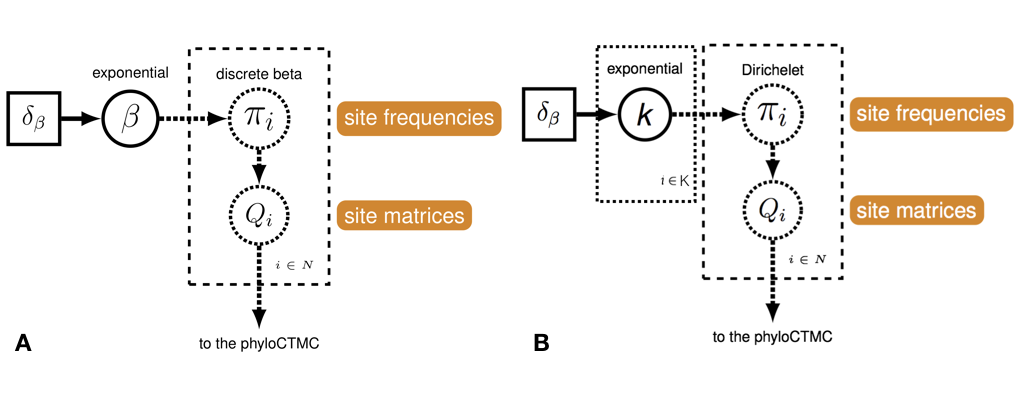
\includegraphics[scale=0.35]{fig/1AB}
\end{figure} 


\begin{figure}
  \caption{Marginal likelihood calculations for the eight models tested for teach of the four empirical datasets. The number of categories into which the Beta (binary data) or Dirichlet (multistate data) is discretized is indicated on the x-axis. Note that due to differing dataset sizes, each plot has a unique y-axis.}
    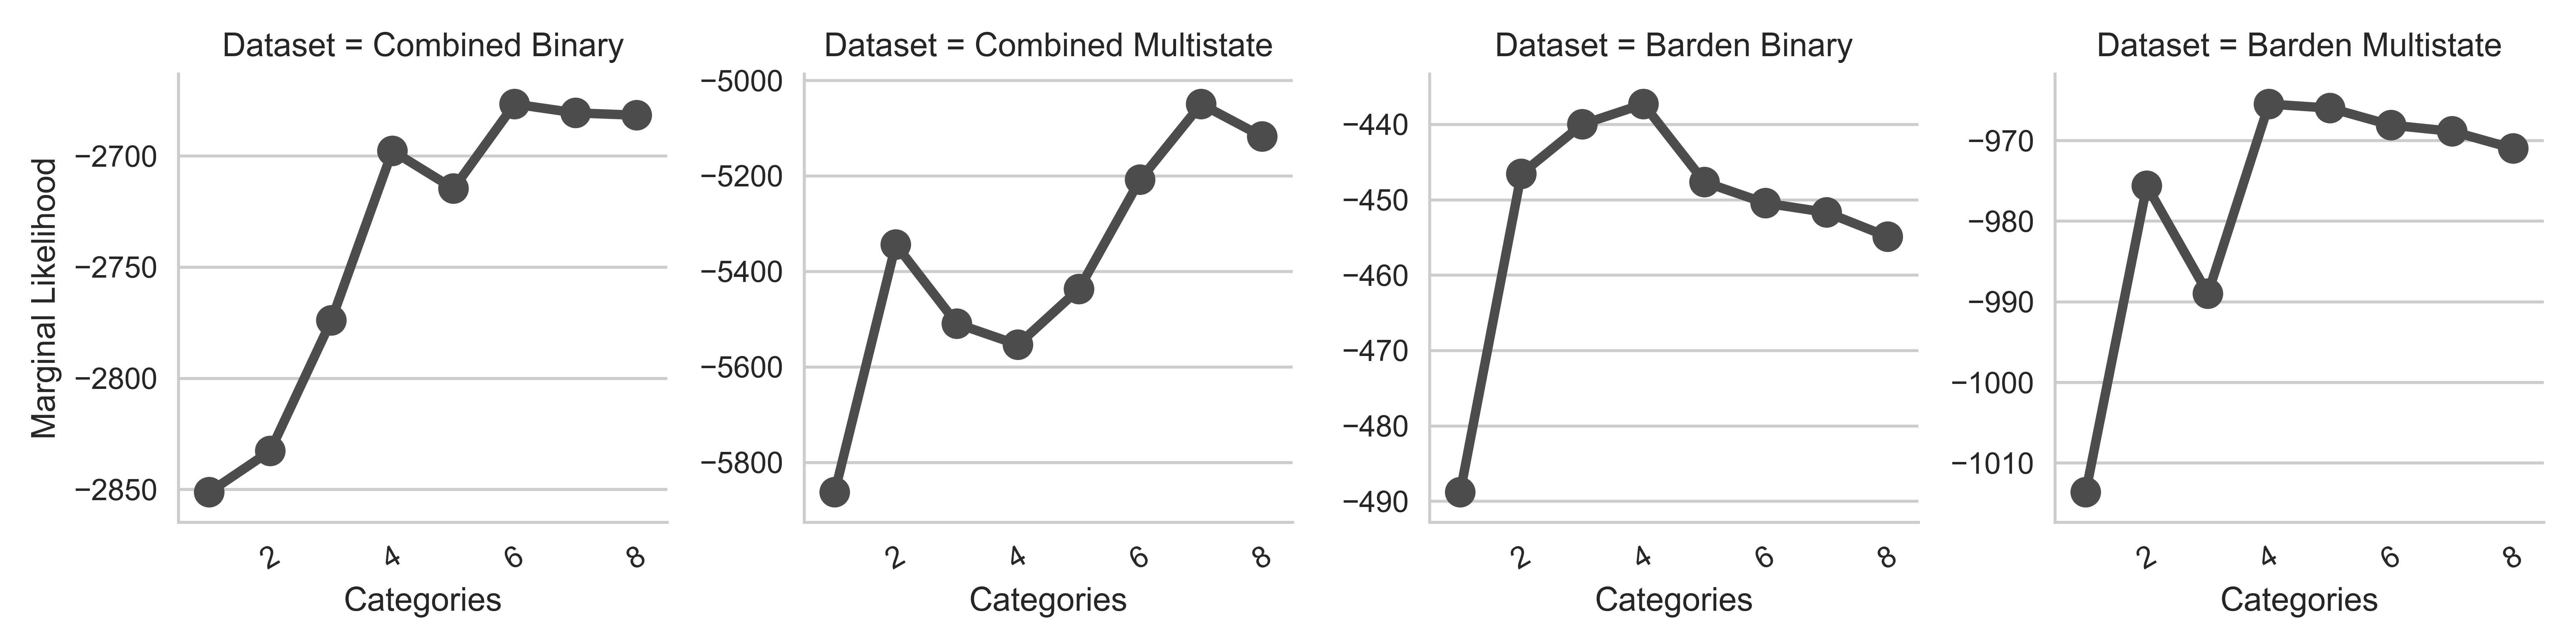
\includegraphics[scale=0.5]{fig/SS_plot_nostar}
\end{figure} 


\begin{figure}
  \caption{Accuracy of phylogenetic estimation in large (135 taxa, 163 character) simulated binary datasets under the Beta model, with 4 discrete categories. Underparameterized models have a wider spread of accuracy values than appropriately or overparamterized models.} 
    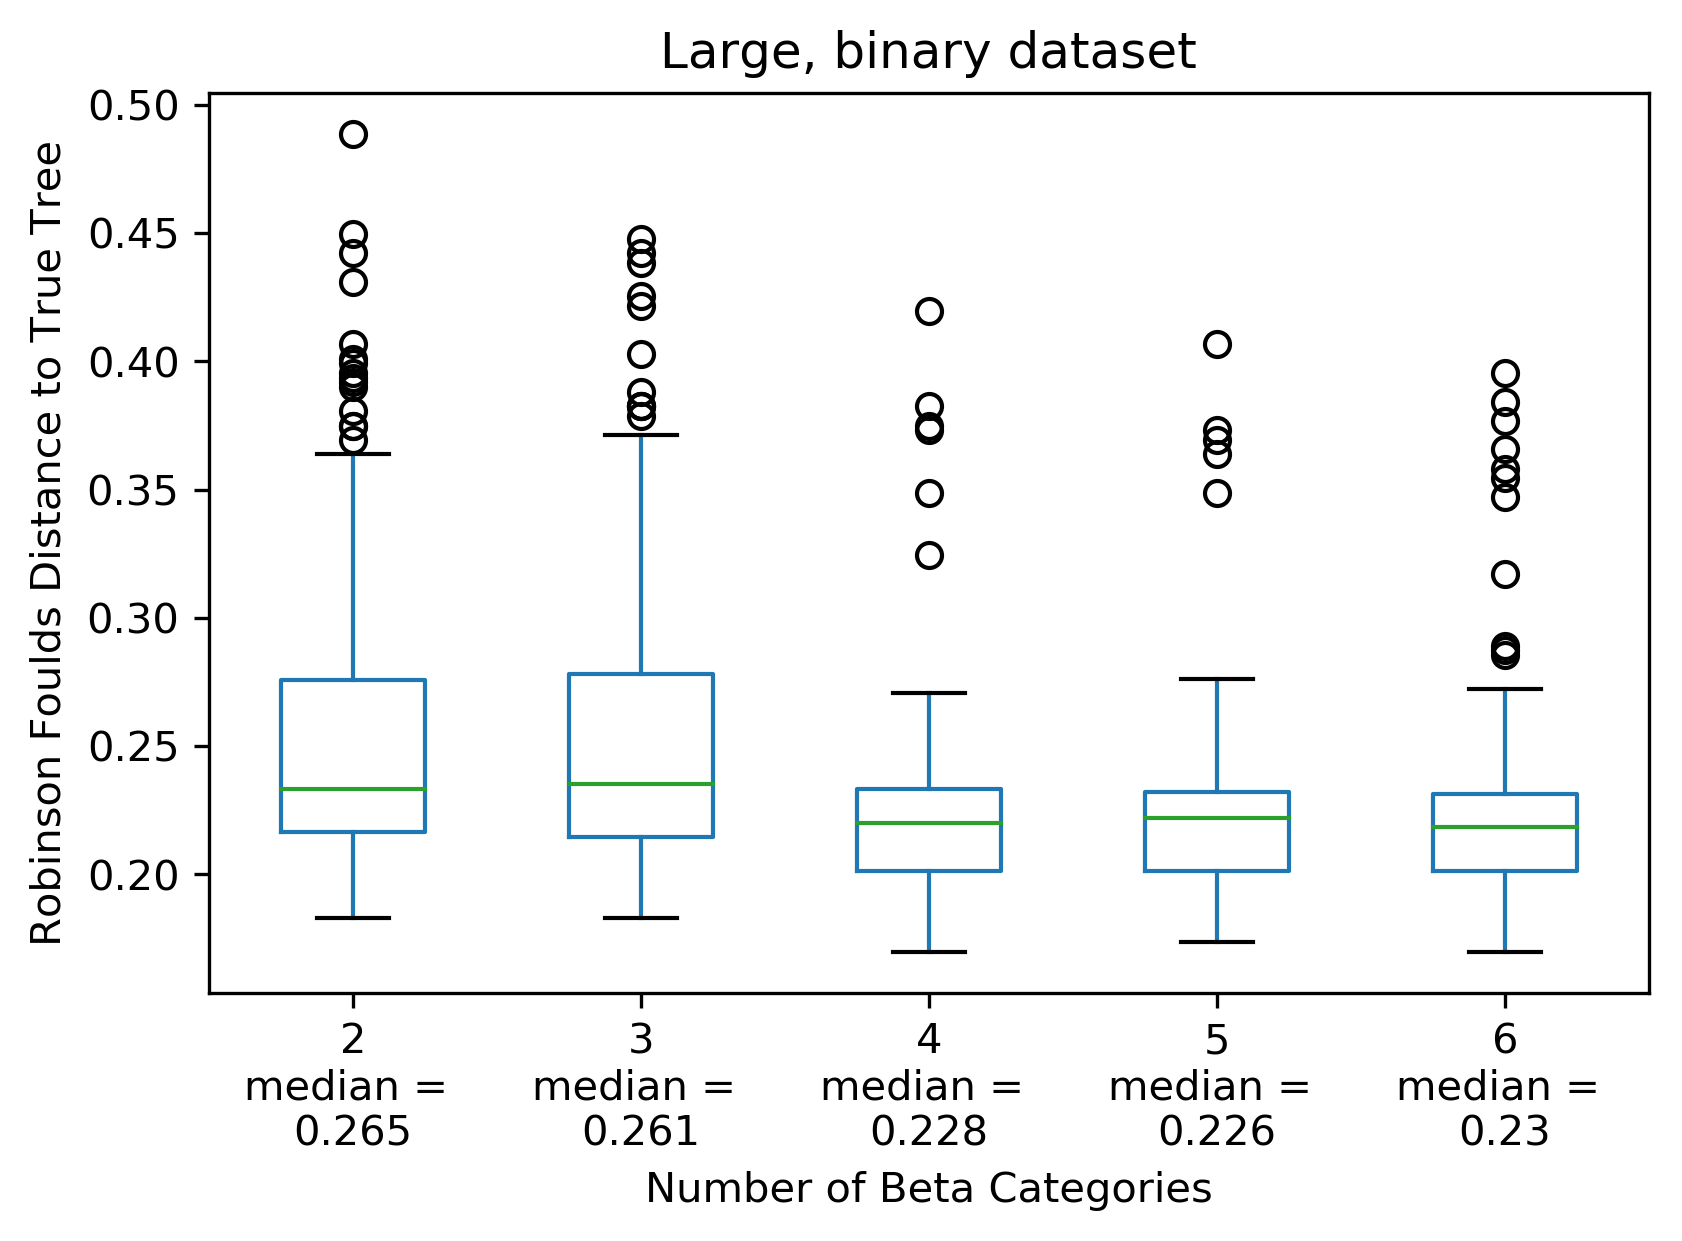
\includegraphics{fig/LargeBinary}
\end{figure} 


\begin{figure}
  \caption{Accuracy of phylogenetic estimation in small (41 taxa, 26 characters) simulated binary datasets under the Beta model. The correct number of simulation categories is 4. In datasets this size, there does not seem to be a relationship between parameterization and accuracy. } 
    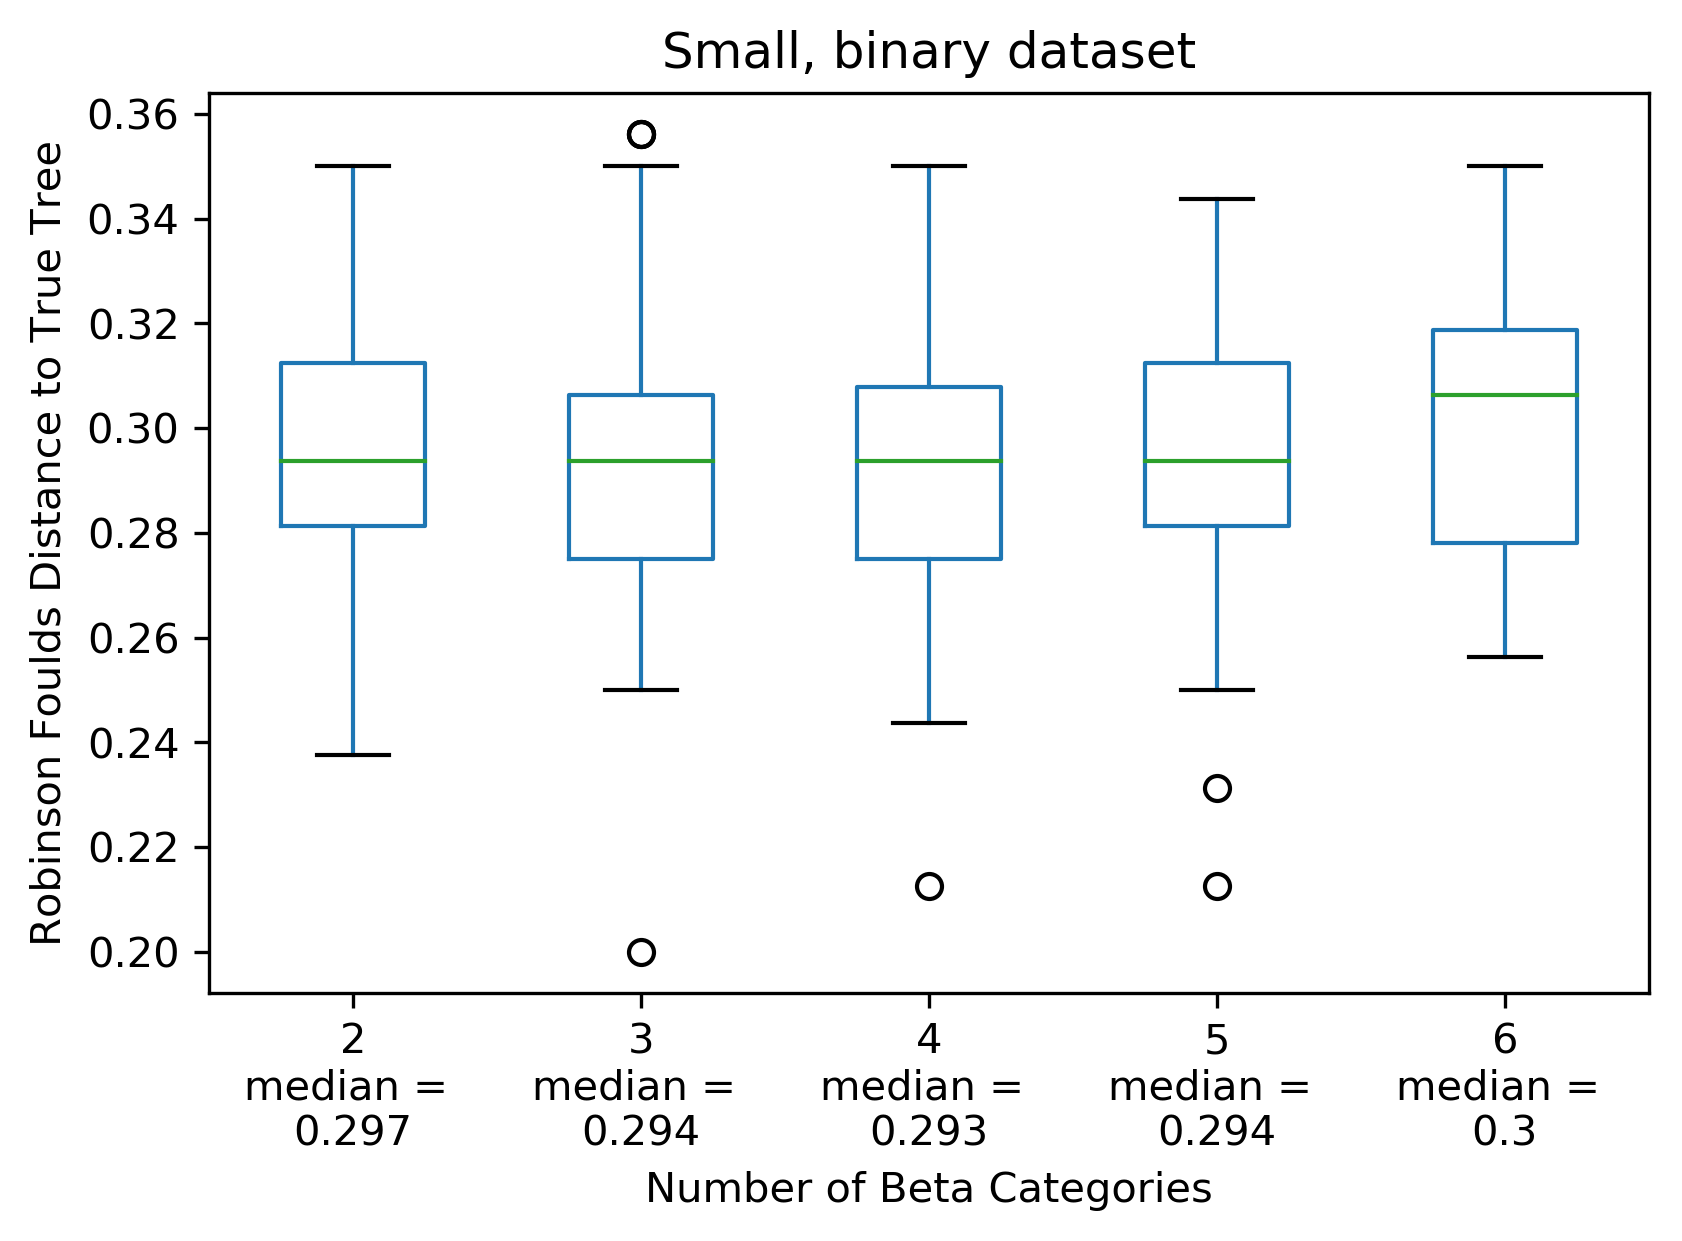
\includegraphics{fig/SmallBinary}
\end{figure} 


\begin{figure}
  \caption{Accuracy of phylogenetic estimation in small large (135 taxa, 163 character) simulated multistate datasets under the SHDM with four transition rate asymmetry categories. Both over- and underparameterization appear to be detrimental to accuracy, though underparamterization is worse.} 
    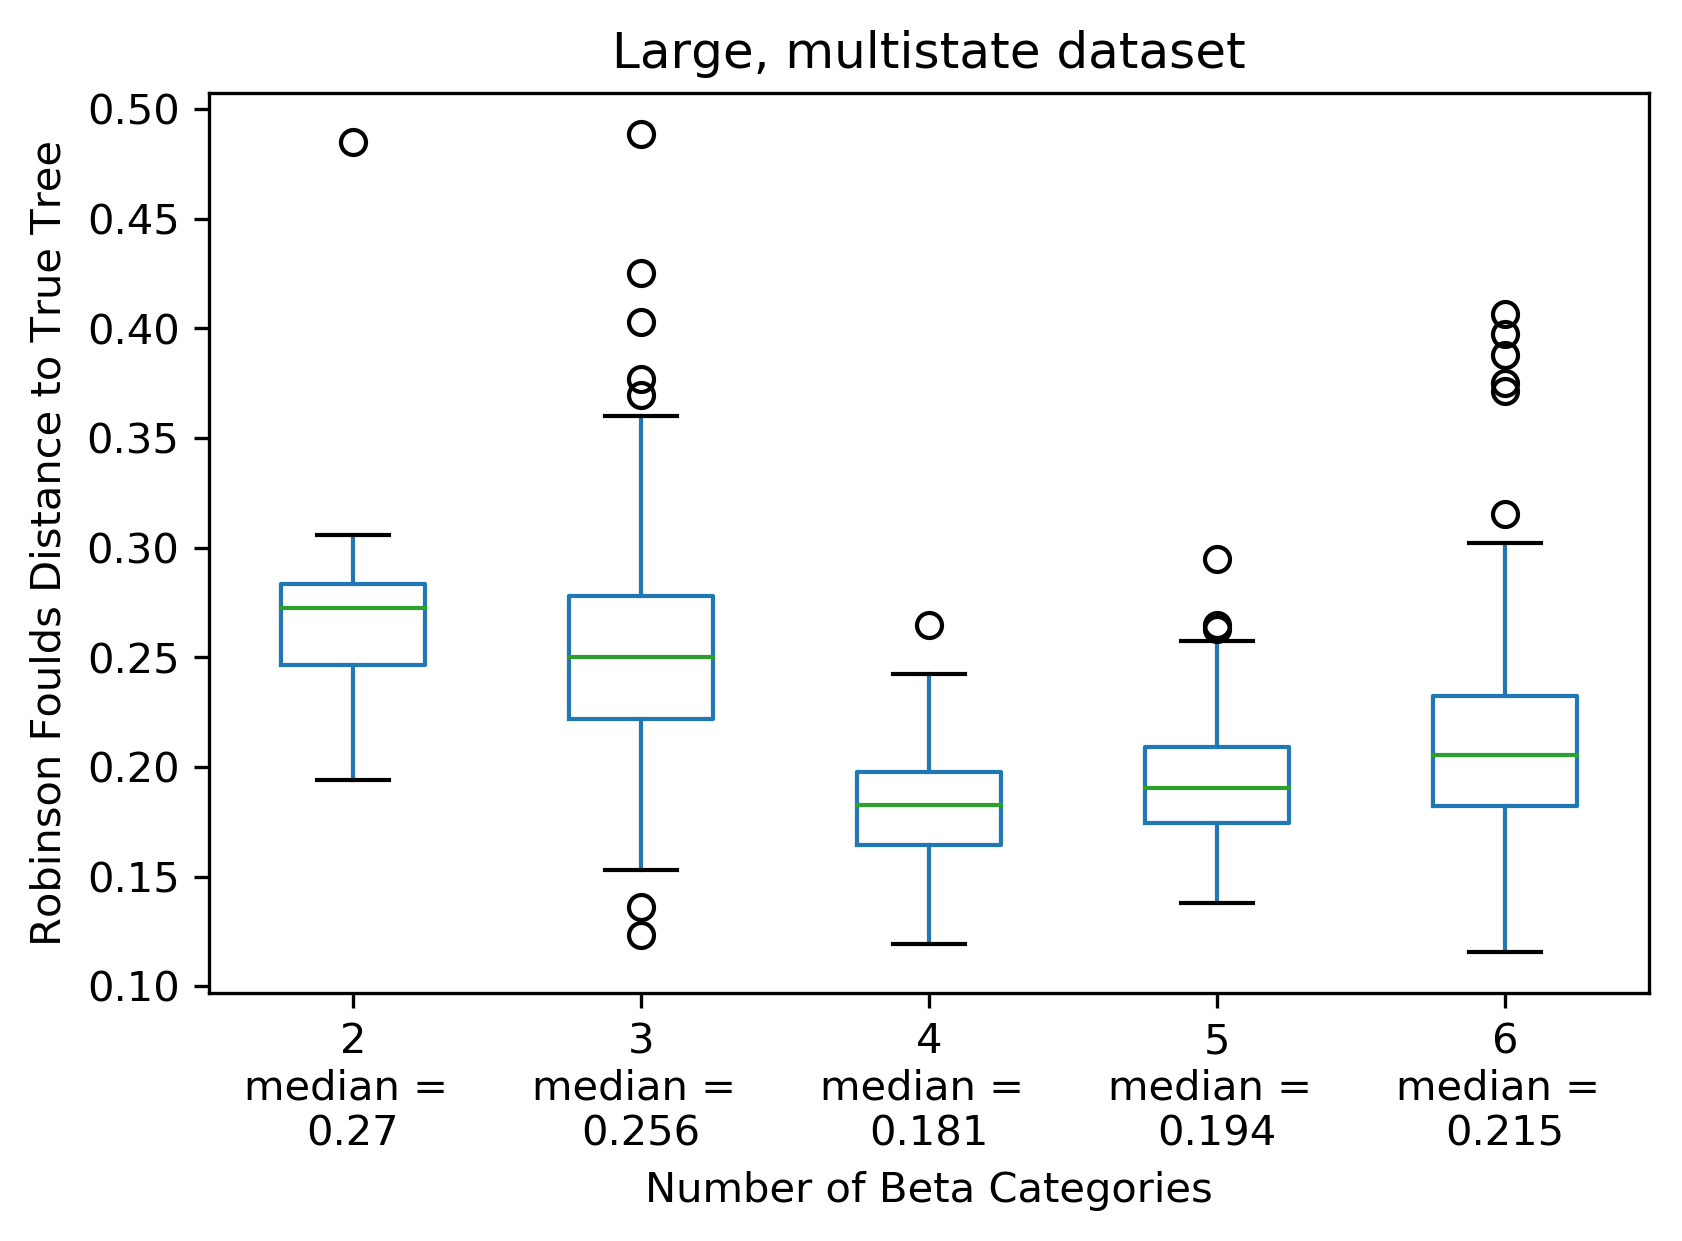
\includegraphics{fig/LargeMultiState}
\end{figure} 

\begin{figure}
  \caption{Accuracy of phylogenetic estimation in small (41 taxa, 26 characters) simulated multistate datasets under the SHDM. The correct number of simulation categories is 4. Much as in the large, binary dataset, underparameterization appears to be more detrimental than overparameterization.} 
    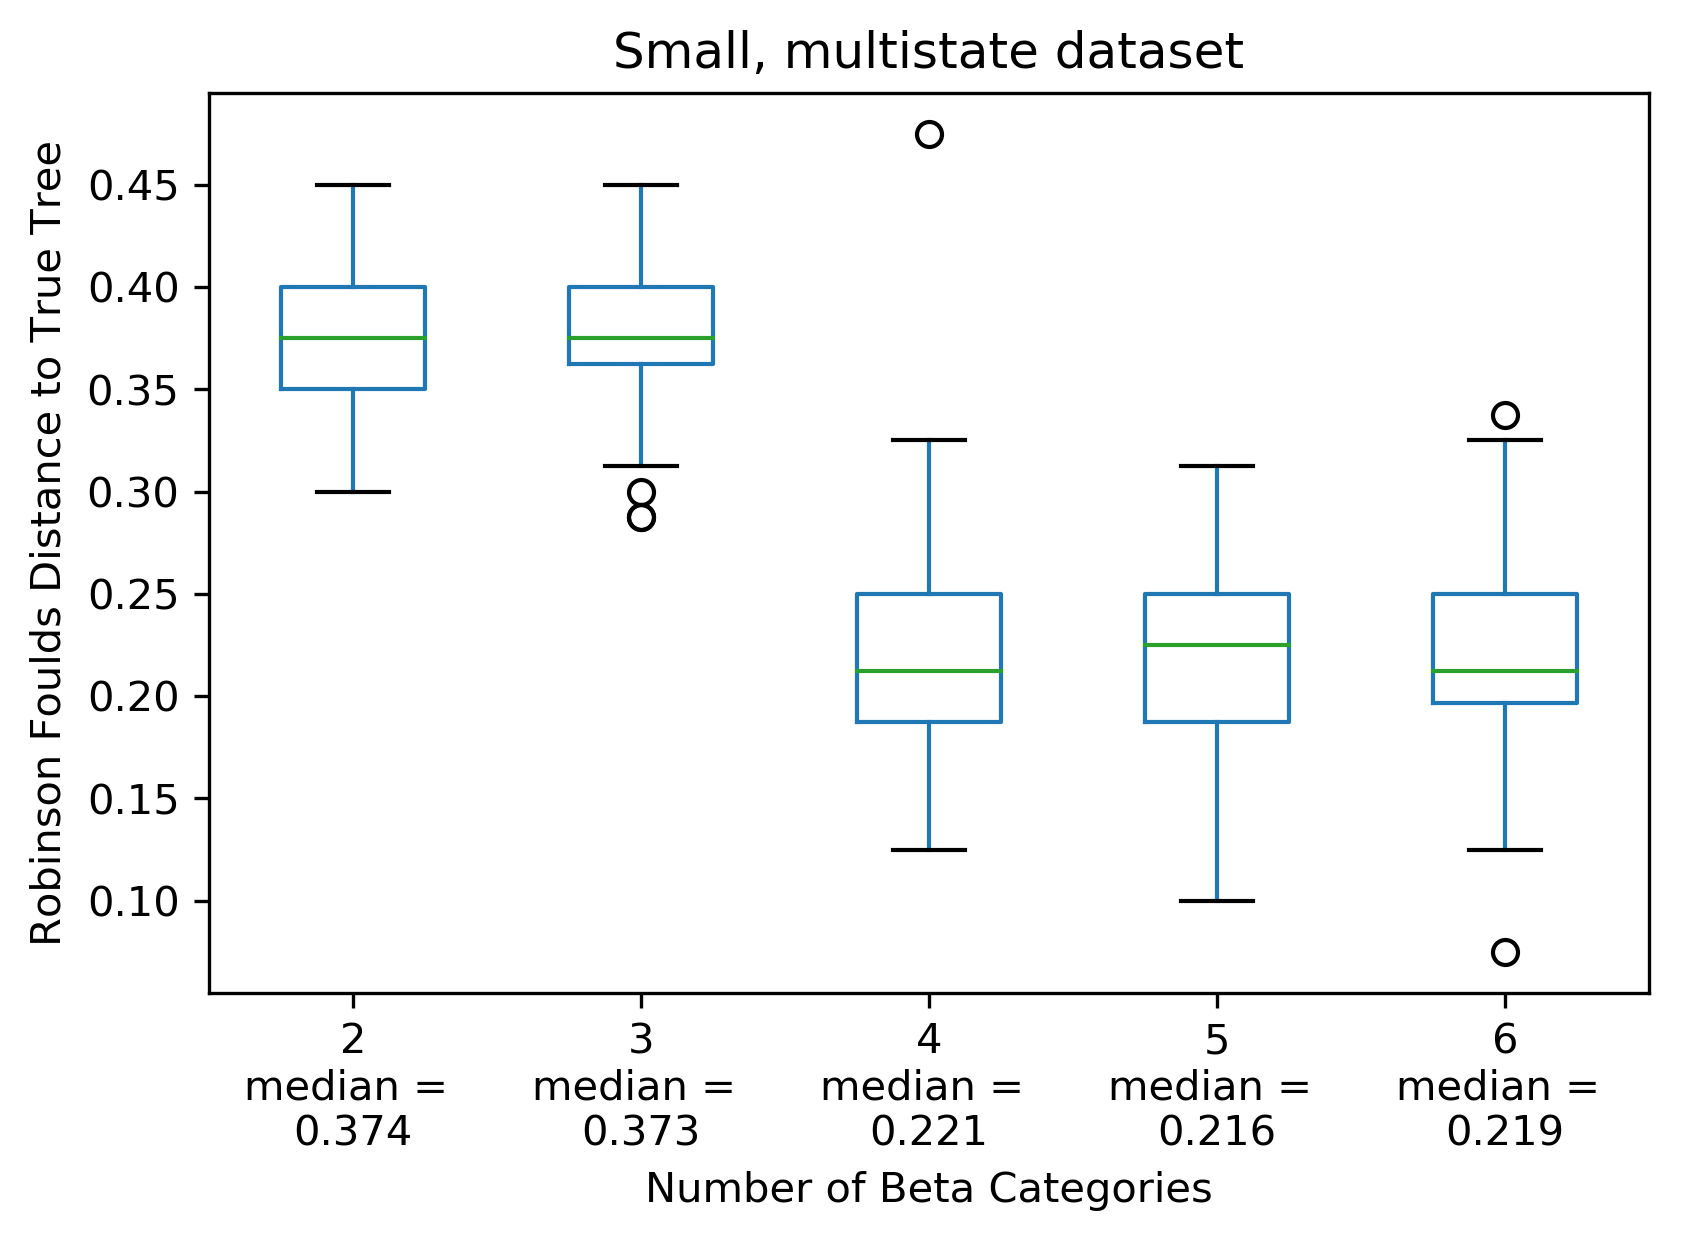
\includegraphics{fig/SmallMS}
\end{figure} 



\end{document}